\documentclass{article}
\usepackage[utf8]{inputenc}
\usepackage[croatian]{babel}
\usepackage{graphicx}


\begin{document}
	\title{Pomoć pri odabiru programskog jezika uz pomoć dijagrama utjecaja}
	\author{Josip Užarević\\\\
		\textit{Ekspertni sustavi}\\\\
		Fakultet elektrotehnike i računarstva\\
		Sveučilište u Zagrebu}
	\date{Siječanj 2017}
	
	\clearpage\maketitle
	\thispagestyle{empty}
	\pagebreak
	
	\tableofcontents
	\thispagestyle{empty}
	\pagebreak
	\setcounter{page}{1} 
	
	\section{Uvod}
	Pri započinjanju implementacije nekakvog projekta, bilo u akademske svrhe ili u profesionalnom smislu, student ili radnik katkad će se zapitati: \textit{Koji programski jezik upotrijebiti? S obzirom na moje predznanje, hoće li mi odabir X uzeti previše vremena? Budući da se radi o arhitekturi Klijent-Poslužitelj, koji mi je programski jezik za poslužiteljsku aplikaciju pametno odabrati?} Zaista, u moru programskih jezika koji su danas u upotrebi, teško je odabrati onaj koji će se programeru ispostaviti kao najisplativiji / najlakši / najupotrebljiviji ili nešto drugo.
	
	U tu svrhu, u okviru projekta na kolegiju \textit{Ekspertni sustavi}, javila se ideja za ostvarenje ekspertnog sustava koji će davati pomoć pri ovom, teškom odabiru. Ekspertni sustav je upravo odličan odabir za rješavanje ovog problema, jer je moguće direktno iskoristiti ekspertno (samim time moguće i subjektivno) znanje u sustav, a uz to dobiti i \textit{ne-diskretne} odgovore (umjesto odgovora \textit{DA/NE}, dobivaju se vjerojatnosni odgovori).
	
	\section{Ekspertno znanje}
	Ekspertno znanje je stečeno isključivo iskustvom autora ovog rada, koje je pak stečeno dugogodišnjom praksom, kako u fakultetske, tako i u profesionalne svrhe te praćenjem \textit{programerske scene}. Samim time raste vrijednost ubačenog ekspertnog znanja, budući da u rad nisu ubačene nekakve gotove vrijednosti dohvaćeni s raznih web-portala ili slično.
	
	\section{Model ekspertnog sustava}
	Za implementaciju ekspertnog sustava odabran je model \textit{mreže utjecaja\textit{}}, koja modelira upravo međusobne utjecaje varijabli te, kao (relativno) završne čvorove može sadržavati i čvorove korisnosti. U danom modelu, varijable koje korisnik može unositi su ustvari \textit{čvorovi izglednosti}, dok su takoreći izlazne vrijednosti upravo \textit{čvorovi korisnosti}. Izgled mreže prikazan je na slici \ref{fig:mreza}.
	
	\begin{figure}
		\centering
		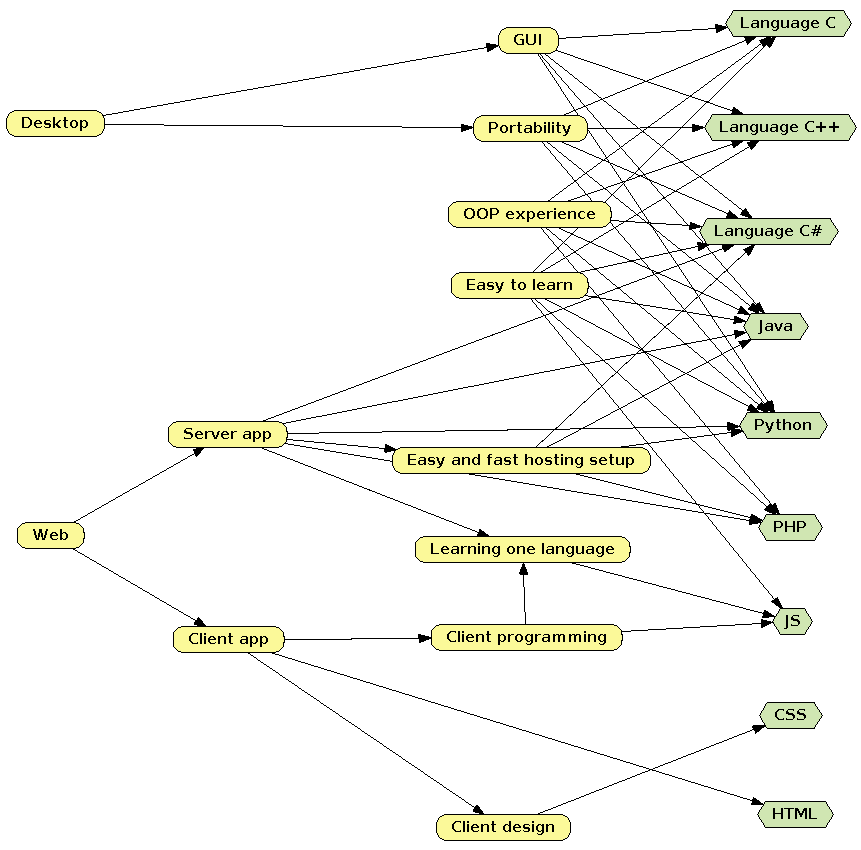
\includegraphics[width=0.9\linewidth]{img/mreza}
		\caption[Model mreže utjecaja]{Model mreže utjecaja za problem određivanja programskog jezika za učenje}
		\label{fig:mreza}
	\end{figure}
	
	Svakom čvoru izglednosti su definirane uvjetne vjerojatnosti za njegove \textit{roditeljske čvorove}. Prvotno su i čvorovima korisnosti bile dodjeljivane tablice vjerojatnosti, no kako neki čvorovi korisnosti imaju čak 6 ulaza, tako su njihove tablice vjerojatnosti imale $ 2^6=64 $ unosa. Zbog ovoga nastaje problem, ne samo u količini posla prilikom unosa, nego još više u unošenju šuma u cijeli sustav. Naime, vrlo teško ekspert može pretpostavljati vjerojatnosti za toliki broj kombinacija samo za jedan čvor, a da ne unese kontradiktorne podatke, kako unutar samog čvora, tako i unutar cijele mreže.
	
	Stoga, čvorovi korisnosti su izvedeni kao linearna kombinacija svih ulaza. Za svaki ulaz ekspert unosi \textit{ocjenu} od -5 do -5, pri čemu je -5 ekvivalentno izjavi \textit{ ulaz negativno utječe na izbor ovog jezika}, +5 \textit{ulaz pozitivno utječe na izbor ovog jezika}, dok je unos nule jednak izjavi \textit{ulaz ne utječe na izbor ovog jezika.} Ovakav izbor funkcije korisnosti se ustvari pokazao kao jako dobar, jer se ujedno pri postupku zaključivanja sustava jasno vidi i raspon svakog izlaza te samim time i \textit{apriori} preferenciju odabira jezika.
	
	\subsection{Unesene vrijednosti u model}
	Slijedi detaljan prikaz unesenih uvjetnih vjerojatnosti u čvorove izglednosti. Kod specifičnih slučajeva bit će navedeni razlozi i ishodi odabira upravo takvih vjerojatnosti. Čvorovi za koje nisu prikazane tablice su čvorovi bez roditelja - njihova razdioba je \textit{apriori} uniformna. Mreža se ugrubo može podijeliti na tri dijela:
	\begin{enumerate}
		\item \textbf{Desktop dio} Ovaj dio mreže je zadužen za osnovno opredjeljenje ka desktop aplikacijama;
		\item \textbf{Web dio} Ovaj dio mreže je zadužen za osnovno opredjeljenje ka web aplikacijama;
		\item \textbf{Općeniti dio} Ovaj dio mreže je univerzalan, bez obzira na osnovno opredjeljenje.
		
	\end{enumerate}
	
	\subsubsection{Desktop dio}
	
	U tablici \ref{fig:gui_p}, ovakvim odabirom tablice, postignuto je to da ukoliko je odabran GUI, onda je nužno odabran i Desktop. Ako je odabran \textit{NE-}GUI, tada je odabran i \textit{NE-}Desktop. Ovime je jednoznačno određeno da je bespredmetno uzimati u obzir razvoj GUI-a ako se neće izrađivati Desktop aplikacija. Situacija je slična i u slučaju portabilnosti, kao i nekih drugih čvorova u mreži.
	
	\begin{table}[h]
		\centering
		\begin{tabular}{ r || r | r }
			Desktop	& Ne & Da \\ \hline
			$ P(\textnormal{GUI = Da} | \textnormal{Desktop}) $ & 0 & 0.5 \\
			$ P(\textnormal{GUI = Ne} | \textnormal{Desktop}) $ & 1 & 0.5 \\
			
		\end{tabular}
		\caption{$ P(\textnormal{GUI} | \textnormal{Desktop}) $}
		\label{fig:gui_p}
	\end{table}
	
	\begin{table}[h]
		\centering
		\begin{tabular}{ r || r | r }
			Desktop	& Ne & Da \\ \hline
			$ P(\textnormal{Portability = Da} | \textnormal{Desktop}) $ & 0 & 0.5 \\
			$ P(\textnormal{Portability = Ne} | \textnormal{Desktop}) $ & 1 & 0.5 \\
			
		\end{tabular}
		\caption{$ P(\textnormal{Portability} | \textnormal{Desktop}) $}
		\label{fig:portability_p}
	\end{table}
	
	\subsubsection{Web dio}
	U web dijelu osnovna podjela je na razvoj poslužiteljske i klijentske aplikacije, koja djelomično razdvaja neke daljnje čvorove (npr. \textit{Easy and fast hosting setup}), dok se na nekim čvorovima stapaju \textit{Learning one language}.
	
	\begin{table}[h]
		\centering
		\begin{tabular}{ r || r | r }
			Web	& Ne & Da \\ \hline
			$ P(\textnormal{Server app = Da} | \textnormal{Web}) $ & 0 & 0.5 \\
			$ P(\textnormal{Server app = Ne} | \textnormal{Web}) $ & 1 & 0.5 \\
			
		\end{tabular}
		\caption{$ P(\textnormal{Server app} | \textnormal{Web}) $}
		\label{fig:server_app_p}
	\end{table}
	
	\begin{table}[h]
		\centering
		\begin{tabular}{ r || r | r }
			Web	& Ne & Da \\ \hline
			$ P(\textnormal{Client app = Da} | \textnormal{Web}) $ & 0 & 0.5 \\
			$ P(\textnormal{Client app = Ne} | \textnormal{Web}) $ & 1 & 0.5 \\
			
		\end{tabular}
		\caption{$ P(\textnormal{Client app} | \textnormal{Web}) $}
		\label{fig:client_app_p}
	\end{table}
	
	\begin{table}[h]
		\centering
		\begin{tabular}{ r || r | r }
			Server app	& Ne & Da \\ \hline
			$ P(\textnormal{Easy and fast hosting setup = Da} | \textnormal{Server app}) $ & 0 & 0.5 \\
			$ P(\textnormal{Easy and fast hosting setup = Ne} | \textnormal{Server app}) $ & 1 & 0.5 \\
			
		\end{tabular}
		\caption{$ P(\textnormal{Easy and fast hosting setup} | \textnormal{Server app}) $}
		\label{fig:easy_and_fast_p}
	\end{table}
	
	\begin{table}[h]
		\centering
		\begin{tabular}{ r || r | r }
			Client app	& Ne & Da \\ \hline
			$ P(\textnormal{Client programming = Da} | \textnormal{Client app}) $ & 0 & 0.5 \\
			$ P(\textnormal{Client programming = Ne} | \textnormal{Client app}) $ & 1 & 0.5 \\
			
		\end{tabular}
		\caption{$ P(\textnormal{Client programming} | \textnormal{Client app}) $}
		\label{fig:client_prog_p}
	\end{table}
	
	Slučaj prikazan u tablici \ref{fig:learning_one_p} je zanimljiv, jer opisuje slučaj ako korisnik želi i poslužiteljski i klijentski dio programirati u jednom jeziku. Jezik \textit{JavaScript} uz korištenje \textit{frameworka} \textit{Node.js} omogućava upravo to. Međutim, razvoj klijenta ne uključuje nužno programiranje (\textit{JavaScript}) ukoliko se npr. radi statička web stranica. Stoga, ovom čvoru je najveća vjerojatnost ukoliko su odabrani klijentsko programiranje i poslužiteljska aplikacija. Ukoliko nijedan od ova dva čvora nije odabran, programiranje u jednom jeziku gubi smisao te je tada vjerojatnos jednaka nuli.
	
	\begin{table}[h]
		\centering
		\begin{tabular}{ r || r | r | r | r }
			Client programming & Ne & Ne & Da & Da  \\ \hline
			Server app & Ne & Da & Ne & Da  \\ \hline
			$ P(\textnormal{Learning one language = Da} | \textnormal{Client programming},\textnormal{Server app} ) $ & 0 & 0.5 & 0.5 & 0.75 \\
			$ P(\textnormal{Learning one language = Ne} | \textnormal{Client programming},\textnormal{Server app} ) $ & 1 & 0.5 & 0.5 & 0.25 \\
			
		\end{tabular}
		\caption{$ P(\textnormal{Client programming} | \textnormal{Client app}) $}
		\label{fig:learning_one_p}
	\end{table}
	
	\begin{table}[h]
		\centering
		\begin{tabular}{ r || r | r }
			Client app	& Ne & Da \\ \hline
			$ P(\textnormal{Client design = Da} | \textnormal{Client app}) $ & 0 & 0.5 \\
			$ P(\textnormal{Client design = Ne} | \textnormal{Client app}) $ & 1 & 0.5 \\
			
		\end{tabular}
		\caption{$ P(\textnormal{Client design} | \textnormal{Client app}) $}
		\label{fig:client_design}
	\end{table}
	
	\subsection{Korisnosti}
	Korisnosti odabira pojedinog programskog jezika, kao što je ranije rečeno, dobivene su unosom koeficijenata za svaki čvor koji je spojen s određenim programskim jezikom.
	
	\section{Proces zaključivanja}
	
	Na slici \ref{fig:inference} prikazano je zaključivanje za primjer odabira Desktop GUUI aplikacije, s objektno orijentiranom paradigmom, da je jezik lako za naučiti te da je portabilnost nebitna. Najviše je bodovan Python, Java i C\#, a najmanje C, što je i logično.
	
	\begin{figure}
		\centering
		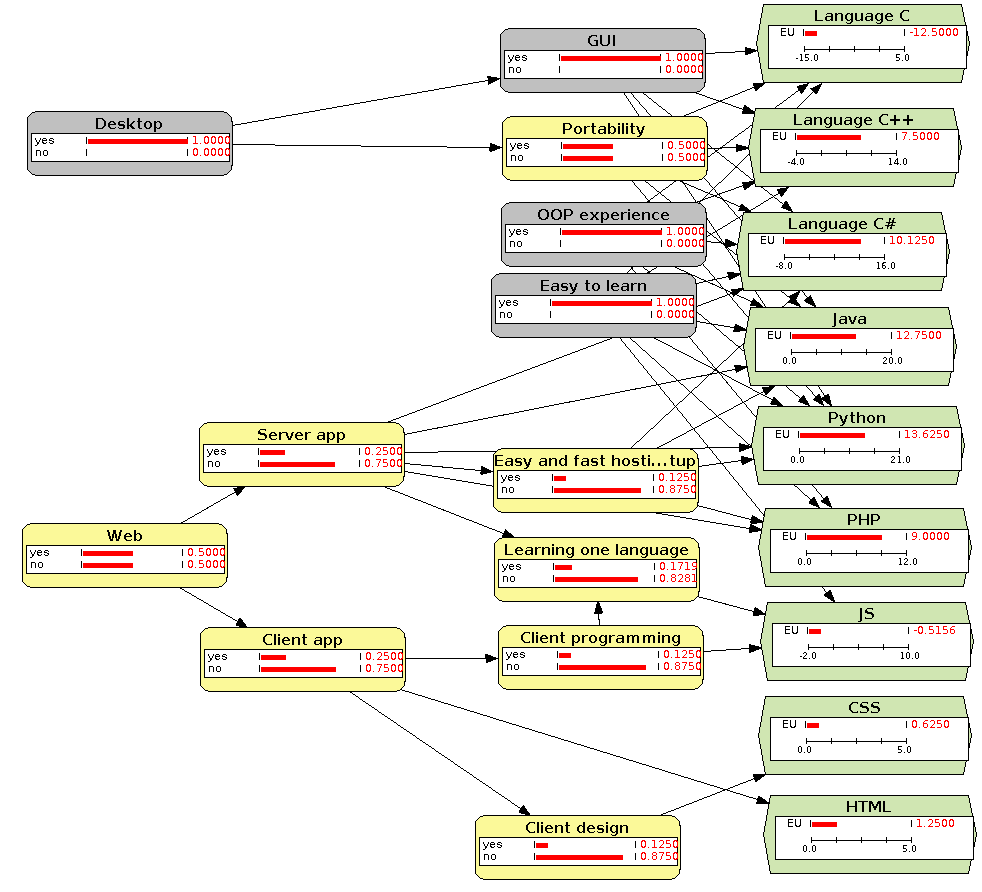
\includegraphics[width=0.9\linewidth]{img/inference}
		\caption[Primjer zaključivanja]{Primjer zaključivanja za odabrane čvorove \textit{Desktop=Da, GUI=Da, OOP experience=Da, Easy to learn=Da}}
		\label{fig:inference}
	\end{figure}
	
	\section{Programska podrška}
	Za realizaciju mreže korišten je alat OpenMarkov, nakon dugog traženja besplatnog programa, a da ima funkcionalnost modeliranja Bayesovih mreža i mreža utjecaja.
	
	\section{Zaključak}
	Izgradnja ekspertnog sustava pomoću Bayesovih mreža i njenih derivata je izuzetno zanimljiva, intuitivna te je proizvod naposljetku jednostavan za korištenje. Međutim, ne postoji besplatan \textit{state-of-the-art} program pomoću kojeg se može vršiti ovakvo modeliranje, a da program radi besprijekorno.
		
\end{document}
